\chapter{PDFBox}

Le site web comprend une partie permettant aux éleves de consulter des documents
en ligne, mis à disposition par les conférenciers.
Les étudiants peuvent soit récupérer les pdf, soit visionner en ligne des "diapositives".
Ces dernières correspondent à des pages de fichiers pdf qui ont été au préalable converties en image. 

Cela a été possible en utilisant un projet open source du nom de PDFBox \cite{pdfbox}.

    \begin{figure}[h]
        \begin{center}
            
\includegraphics[scale=0.6]{images/PDFBox.png} 
        \end{center}

        \caption{Logo PDFBox}
        \label{Logo PDFBox}
    \end{figure}

    \section{Avant propos}

Lors de la mise en place du site web, il nous a été demandé d'implémenter un 
système permettant de fournir des cours au format pdf si les auteurs autorisent
leur diffusion. Dans le cas contraire, une solution devait permettre de les présenter sous forme de diapositives.
La diffusion des cours permet aux éleves d'obtenir les cours assez facilement mais,
ces cours ne sont pas destinés à être imprimés, mais seulement à être visionnés,
c'est le principe même d'une diapositive.
    
   \section{Recherches}

Après quelques recherches, nous avons vu qu'il était 
possible de manipuler un document pdf en le parsant. Mais cela nécessitait 
énormement de temps. Nous avons donc opté pour une solution open source
qui, moyennant quelques modifications nous permettrait d'obtenir un résultat
correcte.
Nous avons pour cela étudier plusieurs pistes:

    \begin{itemize}
    \item PDFsam permet de manipuler les pdf. Cela comprend la fusion de 
     fichiers, le découpage, l'extraction de contenu, la rotation de pages.
     Des options plus avancées sont aussi disponibles comme l'encryptage de fichiers
     pdf ou la modifiation des metadata (contenant le nom de l'auteur,
     le titre ou encore le sujet). Mais malgré tout, cela ne nous convenait pas.
     Nous aurions pu choisir de l'utiliser mais il aurait fallu en plus coder un lecteur 
     pdf en ligne.
     \item pdftohtml permet comme son nom l'indique de convertir un pdf 
     vers un format web composé d'une page HTML et CSS. Mais son utilisation était sujette à de nombreux bugs.
     \item jpedal qui aurait fait un bon candidat si son utilisation était gratuite.
     \item itext qui comme PDFsam permet seulement de manipuler les 
     documents pdf.
     \item PDFbox: notre choix s'est porté sur cette bibliothèque car elle embarque une 
     fonction (au stade de développement) qui permet de convertir les pages d'un
     document en image, en plus d'en permettre la manipulation.
    \end{itemize}

    \section{Présentation du projet PDFBox}

PDFBox est une bibliothèque open source codée en java, permettant de manipuler 
des documents pdf. Elle permet de manipuler les fichiers PDF de nombreuses façons.
Cette bibliothèque est sous license Apache License v2.0, ce qui en fait un lobiciel libre et open source.

Principales fonctionnalités:

    \begin{itemize}
    %expliquer pk difficile de differencier paragraphe si vraiment necessaire au rapport
    \item Extraction de texte
           Cette fonction est toujours au stade de développement car il est difficile de 
           différencier deux paragraphes différents dans un fichier pdf (la position 
           du texte est donnée par des positions absolues, ce qui permet de disposer 
           le texte exactement à l'emplacement où on le souhaite).
	\item Fusion de documents PDF
	\item Encryptage/Décryptage
	\item Création de PDF depuis un fichier texte
	\item Création d'images à partir d'un document PDF. C'est cette fonction qui nous intéresse.
           C'est cette dernière qui servira à fournir les diapositives que les élèves pourront consulter à partir 
           du site web.
	\item Impression de PDF
	\end{itemize}

Il faut savoir que la fonction convertissant un pdf en images est encore
au stade de développement. Ce qui veut dire que  les fonctionnalités ne sont 
pas encore toutes implémentées ou encore que certains bugs subsistent encore.

Ci-dessous, nous allons expliquer les problèmes que nous avons rencontrés,
ainsi que la manière dont nous avons résolus chacun d'entre-eux.

Avant toute chose, il est important de noter que la résolution à ceux-ci
à été possible grâce à la documentation de PDFBox et à celle de la classe 
java.awt.Font ainsi qu'au débugueur inclus dans l'environnement de dévelopement 
Eclipse.

	\section{MediaBox et CropBox}

Lors de nos tests, nous nous sommes rendues compte qu'il pouvait y 
avoir un problème de conversion avec un fichier pdf contenant à la fois une 
"cropbox" et une "mediabox". Il faut savoir que lors de la visualisation d'un 
document pdf, par défaut, on ne voit que la partie que l'auteur veut que l'on 
voit. Ce procédé est par exemple utilisé dans les imprimeries. 

    \begin{itemize}
    \item La cropbox correspond  à la partie visible par tous du document, 
     c'est celle qui est destinée à être vue.
    \item La mediabox comprend la cropbox et correspond à la totalité 
     réelle du document et non pas seulement à la partie visible 
     lors de la lecture du fichier avec Adobe Reader par exemple. 
    \end{itemize}

    \begin{figure}[h]
        \begin{center}
        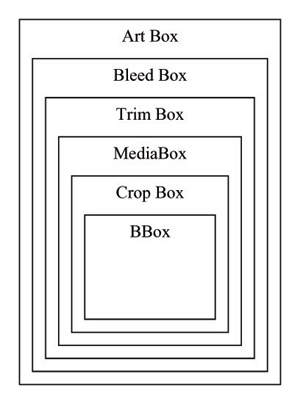
\includegraphics[scale=0.6]{images/boxesInPDF.jpg} 
        \end{center}
        \caption{Hiérarchie des différentes box}
        \label{Hiérarchie des différentes box}
     \end{figure} 

Ce premier problème se rapporte au fait de ne pas pouvoir convertir
une page en entier si une cropbox était spécifiée (la médiabox l'est 
obligatoirement elle). Pour cela, il a fallu envoyer les bonnes dimensions 
de pages à chaque fois qu'une image est créée, et cela sans utiliser la fonction
getcropbox retournant un objet de type PDRectangle et qui ne fonctionne 
pas correctement (lance un null pointeur exception). On a donc changé le
code pour faire appel à la fonction findcropbox() qui elle fonctionne 
    correctement.

	%TODO: Dire quel fichier et quelles lignes on été modifiés

    \lstset{language=Java}
    \begin{lstlisting} 
    private static void changeCropBoxes(PDDocument document,float a, float b, float c,float d)
    {
	List <PDPage> pages = document.getDocumentCatalog().getAllPages();
	for( int i = 0; i < pages.size(); i++ )
	{
        System.out.println("resizing page");
        PDPage page = (PDPage)pages.get( i );
        PDRectangle rectangle = new PDRectangle();
        rectangle = page.getMediaBox();
        a=0;
        rectangle.setLowerLeftY(a);
        rectangle.setLowerLeftY(b);
        rectangle.setUpperRightX(c);
        rectangle.setUpperRightY(d);

        page.setMediaBox(rectangle);
        page.setCropBox(rectangle);
	 }
    }
    \end{lstlisting}

Une fois que les dimensions recherchées sont récuperées, on les affecte
aux pages du document PDF l'on veut convertir. Ainsi on obtient bien les bonnes 
dimensions de pages.

    \section{Polices embarquées}

Il faut savoir que suivant le software employé pour créer les PDF et
les polices utilisées, il est possible que ces dernières soient directement
inclues dans le fichier final. Cela est autorisé par la norme ISO régissant 
ce type de fichier. Or en interne, la gestion des polices est faite via la 
classe "java.awt.Font". Et malheureusement, cette dernière nécessite de travailler
avec des polices complètes.

Il arrive donc que suivant les fichiers à transformer en images, si la police 
est contenue dedans, le resultats soit illisible, dû à la confusion par rapport
au caractère manquant.

        %TODO: Image de diapositive erronée.

Comme mentionnée précédemment, certains fichiers PDF peuvent contenir eux 
même la définition ainsi que les glyphes correspondants aux caractères utilisés dans 
le document. Cependant, si ces dernières ne sont pas complètes, il subsistait
quelques erreurs.

Nous avons essayé de modifier nous même les polices incriminées mais 
sans résultat probant. Nous avons donc patché le code une deuxième fois 
en donnant la police système si le document en utilisait une interne.

De ce fait, tous les documents se verront écrit avec cette police mais 
on garde l'avantage de garder partiellement le style d'écriture 
(soulignement, couleur, taille).

%TODO: Donner les diffs en annexe
